\section{Transformationsfehler} \label{Fehler bei der Transformation}
In Kapitel \ref{entwicklung} wurde gezeigt wie komplex die Etablierung von Continuous Delivery für Unternehmen ist. Bei diesem Prozess können Probleme auftreten, die in dem Abschnitt diskutiert werden. Es tritt häufig der Fehler auf, dass Unternehmen dazu neigen, Continuous Delivery als einen Endzustand anzusehen und die Mentalität innerhalb der Organisation nicht anpassen. Allgemein lassen sich die Menge der Probleme in die sechs Kategorien Builddesign, Systemmodularisierung, Integration, Testphase, Release, Mensch und Organisationsstruktur klassifizieren. In der Arbeit von Laukkanen et al treten hier 40 Probleme auf (siehe Abbildung \ref{studie}) \cite{Laukkanen.2017}. 

\begin{figure*}[ht]
	\centering
	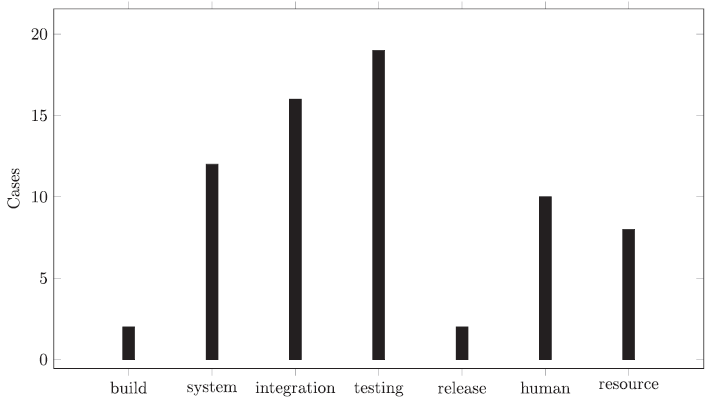
\includegraphics[width=0.8\textwidth,]{images/Transformationproblems}
	\caption{Visualisierung der Probleme der einzelnen Bereiche\cite{Laukkanen.2017}.}
	\label{studie}
\end{figure*}

\subsection{Builddesign} \label{builddesgin}
Bereits die Entscheidung, wie das Builddesign aufgebaut und konfiguriert wird, kann eine zukünftige Problemursache darstellen. Ein Grund hierfür kann die Erstellung von komplexen und unflexiblen Buildskripten sein. Das Builddesign ist dadurch stark an das Zielsystem gekoppelt, sodass minimale Skritpänderungen zu Buildfehlern führen. Dies erfordert intensive Pflege- und Wartungsarbeiten, welche die Einführung einer DevOps-Kultur drosseln. Aber auch stellt die Modellierung des Systems eine Abhängigkeit für das Builddesign dar, da die Auflösung von Abhängigkeiten kritisch sein könnte (zum Beispiel zyklische Abhängigkeiten).

\subsection{Systemmodularisierung}  \label{Systemmodularisierung}
Wie in Abschnitt \ref{builddesgin} aufgezeigt wurde stellt die Systemmodularisierung eine weitere Problemursache dar. Eine geeignete Systemmodellierung führt zu einer autonomen und unabhängigen Entwicklung. Von einer ungeeigneten Architektur ist die Rede, wenn sie monolithisch gekoppelt ist. Eine ungeeignete Systemmodularisierung führt zu einem überhöhten Entwicklungsaufwand, Testbarkeit und Wartbarkeit. Dadurch erhöht sich sowohl die Fehleranfälligkeit des Systems als auch die Code-Inkonsistenz. Daraus folgt, dass sich die Software in einem nicht auslieferbaren Zustand befindet. Jedoch kann auch bei einer geeigneten Architektur Probleme auftreten, indem zu starke Systemmodellierung betrieben wird. Das führt zu einer Erhöhung der Komplexität, sodass neue Teammitglieder die Software schwer weiterentwickeln und warten können \cite{Laukkanen.2017}. 

\subsection{Integration} \label{Integration}
Die Integration umfasst Probleme, die bei der Zusammenführung von Softwarekomponenten entstehen \cite{LianpingEtPaddy.2015}. Sobald diese nicht wie vorgesehen zusammengeführt werden, treten hier Probleme auf. Nicht selten kommt es vor, dass Entwickler einmal täglich Quellcodeänderungen hochladen. Das hat die Folge, dass eine hohe Anzahl von Änderungen mit sich bringt und diese im Konflikt mit anderen Änderungen stehen. Im Fall eines Fehlers im Buildprozess kann der Fehler nicht sofort identifiziert werden und es entsteht eine Arbeitsblockade. Des Weiteren hat diese Vorgehensweise den Nachteil, dass überhöhter Netzwerklatenz erzeugt wird. Eine oft genutzte Methode ist hier das Erstellen von mehreren Abzweigungen des Hauptentwicklungsstrangs. Diese Lösung ist allerdings problembehaftet. Während die Entwicklung am Hauptentwicklungsstrang voranschreitet, divergieren Verzweigungen, sodass die Vereinigung der Stränge zum Problem wird. Die Lösung dieser Viereinigungsprobleme resultiert in mehr Aufwand, was zur einer reduzierten Produktivität führt \cite{Laukkanen.2017}. 

\subsection{Testphase}
Tests sollten eindeutige Validierung vornehmen. Bei bestimmten Tests, wie beispielsweise ''flaky tests'', entstehen hier langwierige Probleme. Bei diesen Tests werden zufällige Resultate erzeugt, die nicht determinierbar sind. Das erschwert die Testphase. Das geht aus dem folgenden Zitat hervor: 

\begin{quote}\glqq ...several of the automated activities do not yield a clear “pass or fail” result... \grqq~\cite[S.65]{Laukkanen.2017}\end{quote}
%

\subsection{Mensch und Organisationsstruktur}
Eine letzte Problemursache ist der Mensch, welcher aktuell die größte Herausforderung darstellt. Die Adaption von Continuous Delivery erwartet wie aufgeführt Agilität und Flexibilität. Das setzt voraus, dass eine Akzeptanz für diese Vorgehensweisen vorhanden ist. Dies stellt die erste Hürde dar, wie im folgenden Zitat zu sehen ist. Sowohl auf Management- als auch Mitarbeiterebene wird Motivation und Disziplin verlangt. Des Weiteren muss erwähnt werden, dass in Softwareteams mehr Druck herrscht, da sich die Software in einem ständig auslieferbaren Zustand befinden muss. Das kann negative Auswirkungen auf die Motivation der Teammitglieder haben und führt gegebenenfalls zu einer angespannten Arbeitsatmosphäre. Aus technischer Sicht verlangt Continuous Delivery sowohl umfangreiches Wissen im Bereich Buildmanagement als auch bei der Programmierung von unterschiedlichen Skripten \cite{Laukkanen.2017}. Das erfordert eine Einarbeitung in die Thematik. 

\begin{quote}\glqq ...But it was hard to convince them that we needed to go through our implementation “hump of pain”to get the pieces in place that would allow us to have continuous integration. I worked on a small team and we didn’t seem to have any “extra”time for me to work on the infrastructure we needed. \grqq~\cite[S.373]{Stolberg.2009} \end{quote}
%

%\begin{figure*}[ht]
%	\centering
%	\includegraphics[width=0.8\textwidth,]{images/all}
%	\caption{Übersicht der Probleme\cite{Laukkanen.2017}.}
%	\label{integrationsprobleme}
%\end{figure*}